\chapter{प्रयोगशाला तकनीकें III: शोध-अभ्यास}\label{ch:b3:lab-techniques-3}

ब्यूटिललिथियम विलयन की बोतल में आग लग जाती है यदि उसकी एक बूँद वायु से मिल जाए; एक
\omterm{def:b3:lab-techniques-3:schlenk}{ग्लवबॉक्स} ऑक्सीजन और जल को प्रति दस लाख कुछ भागों से नीचे रखता है ताकि ऐसे
यौगिकों को खाने के नमक की तरह तौला जा सके। शोध-रसायन प्रायः वायुमंडल को
बाहर रखने से आरंभ होता है, और एक ऐसे दावे के साथ समाप्त होता है जिसे दूसरे
जाँच सकें: एक नया यौगिक, जिसकी संरचना और शुद्धता कई स्वतंत्र विधियों से सिद्ध हो,
और जिसके आँकड़े अभिलिखित और प्रकाशित हों ताकि कार्य को दोहराया जा सके। यह
अंतिम अध्याय शोध के अभ्यास को एकत्र करता है: वायु-संवेदी पदार्थों को सँभालना,
किसी नए यौगिक का अभिलक्षणन, किसी परिणाम का सांख्यिकीय मूल्यांकन,
नोटबुक रखना और साहित्य पढ़ना, और ऐसी प्रक्रिया के जोखिमों का मूल्यांकन
जिसे पहले किसी ने नहीं चलाया।

\begin{recall}
प्रथम वर्ष के खंड ने संकट, जोखिम, चित्रलेख, H और P कथन, सुरक्षा
आँकड़ा पत्रक और मापन अनिश्चितता, उसके A- और B-प्रकार मूल्यांकनों सहित, प्रस्तुत किए;
द्वितीय वर्ष के खंड ने अक्रिय वायुमंडल, उपचार-पश्चात् प्रक्रिया, शुष्कन कारक, फ़्लैश वर्णलेखन,
द्रव्यमान स्पेक्ट्रममिति (HRMS, एकसमस्थानिक द्रव्यमान), $^{13}$C NMR, विश्वास्यता अंतराल,
स्टूडेंट गुणांक, अंशांकन, परिशुद्धता, यथार्थता, अभिनति, पुनरावर्तनीयता,
विधि मान्यकरण, रुद्धोष्म ताप-वृद्धि और तापीय अनियंत्रण।
\Cref{ch:b3:advanced-nmr}, \cref{ch:b3:x-ray-diffraction} और
\cref{ch:b3:electrode-kinetics} ने संरचनात्मक और विद्युतरासायनिक
विधियाँ दीं।
\end{recall}

\begin{omfigure}
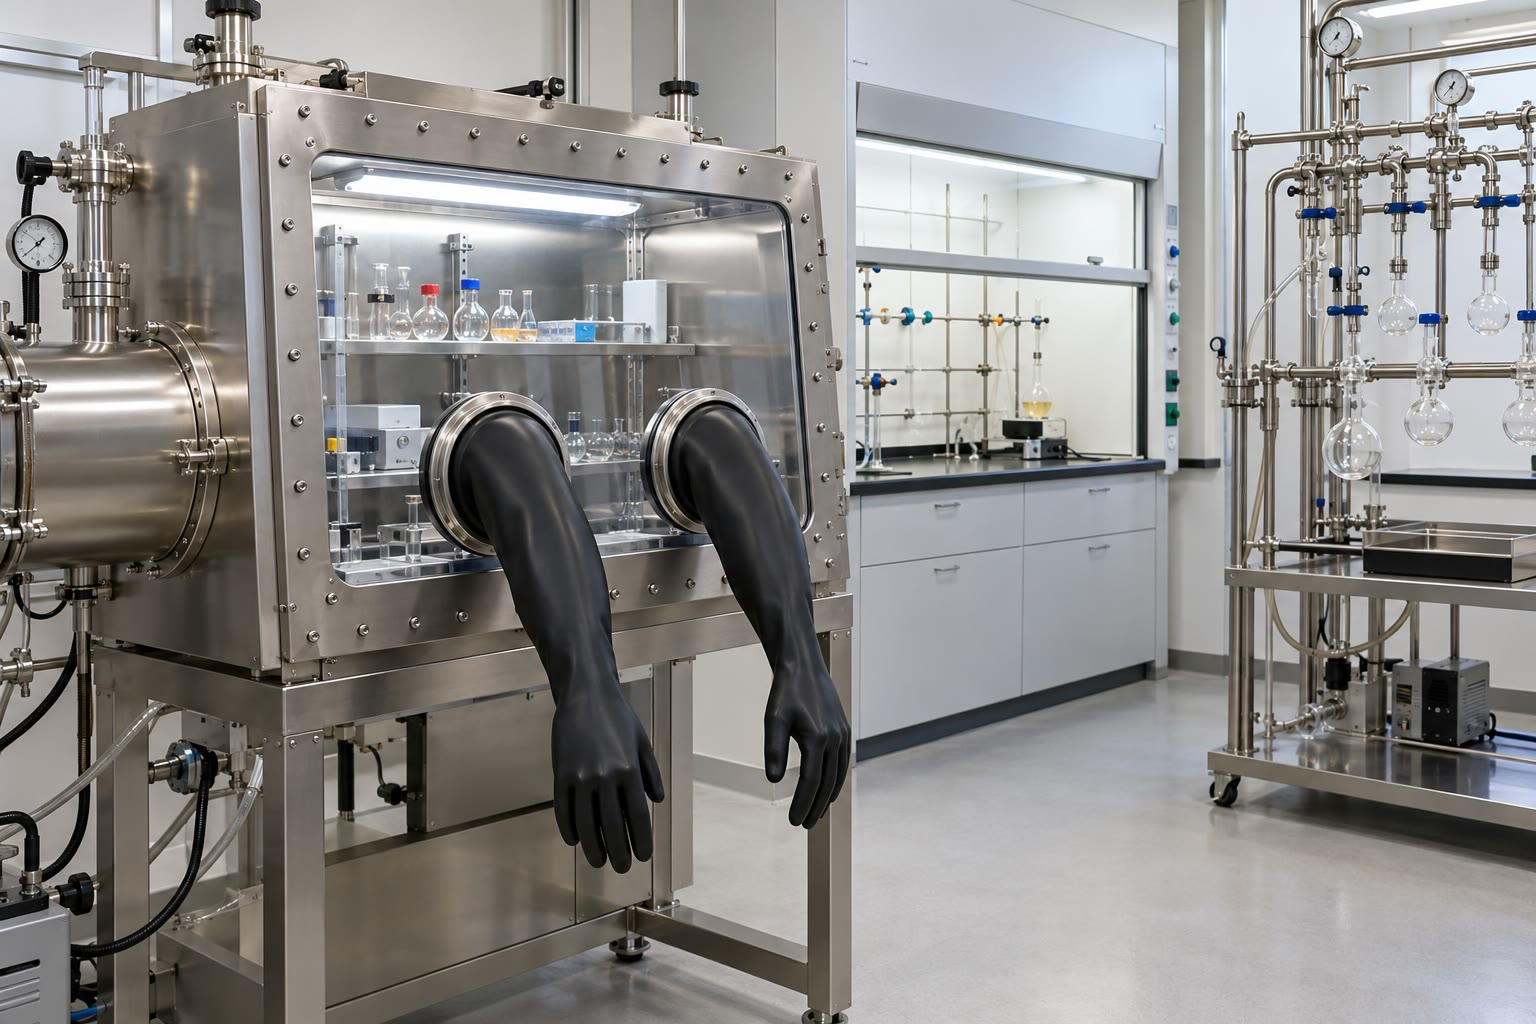
\includegraphics[width=0.58\linewidth]{images/book4/ai/b3-33-glovebox.jpg}

{\small \omterm{def:b3:lab-techniques-3:schlenk}{ग्लवबॉक्स} वाली एक शोध प्रयोगशाला: स्टेनलेस-स्टील की पेटी में, जो शुष्क
नाइट्रोजन या आर्गन से भरी है, दस्तानों से होकर काम किया जाता है; बाईं ओर का
बेलन वस्तुओं को भीतर लाने और बाहर ले जाने का पूर्वकक्ष है।}
\end{omfigure}

\section{वायु के बिना कार्य}

\begin{definition}[वायु-संवेदी यौगिक]\label{def:b3:lab-techniques-3:air-sensitive}
\emph{वायु-संवेदी यौगिक}\index{वायु-संवेदी यौगिक} वायु की डाइऑक्सीजन या जल से
अभिक्रिया करता है, अपघटित होकर या अपनी सक्रियता खोकर। \emph{स्वतःज्वलनशील
पदार्थ}\index{स्वतःज्वलनशील पदार्थ} वायु में स्वतः
प्रज्वलित हो जाता है।
\end{definition}

\begin{definition}[श्लेंक लाइन और ग्लवबॉक्स]\label{def:b3:lab-techniques-3:schlenk}
\emph{श्लेंक लाइन}\index{श्लेंक लाइन} काँच का एक दोहरा बहुशाखी नलिका-तंत्र है, जिसकी एक नली
एक शीत पाश से होकर निर्वात पंप से जुड़ी होती है, दूसरी शुष्क अक्रिय
गैस की आपूर्ति से, जिसका निकास एक तेल बबलर से होता है, और जिसकी टोंटियाँ प्रत्येक निकास-मुख को
किसी एक से जोड़ती हैं। \emph{श्लेंक फ़्लास्क}\index{श्लेंक फ़्लास्क} में लाइन से जोड़ने के लिए
टोंटी-युक्त एक पार्श्व भुजा होती है। \emph{ग्लवबॉक्स}\index{ग्लवबॉक्स} अक्रिय गैस से भरी,
निरंतर शोधित, एक बंद पेटी है, जिसमें दस्तानों से होकर
काम किया जाता है।
\end{definition}

\begin{omfigure}
\begin{tikzpicture}[font=\scriptsize, >=Stealth]
  % manifolds
  \draw[om glass, line width=1.1pt] (0,3.0) -- (8.0,3.0);
  \draw[om glass, line width=1.1pt] (0,2.5) -- (8.0,2.5);
  \node[anchor=east] at (-1.0,3.0) {अक्रिय गैस};
  \node[anchor=east] at (0,2.5) {निर्वात};
  % taps
  \foreach \x in {2.0,4.0,6.0} {
    \draw[om glass] (\x,3.0) -- (\x,2.5);
    \draw[fill=white] (\x,2.75) circle (0.12);
    \draw (\x-0.1,2.75) -- (\x+0.1,2.75);
    \draw[om glass] (\x,2.5) -- (\x,2.0);
  }
  % flask on the middle tap
  \draw[thick, black!60] (4.0,2.0) -- (4.0,1.6) -- (4.6,1.6);
  \pic[scale=0.5, transform shape] at (5.0,-0.2) {rbflask={0.3}{omDef!20}};
  \draw[om glass] (4.6,1.6) -- (4.9,1.25);
  \node[anchor=west] at (5.4,0.4) {श्लेंक फ़्लास्क};
  % bubbler at the gas end
  \pic[scale=0.55, transform shape] at (8.9,1.5) {bubbler};
  \draw[om glass] (8.0,3.0) -- (8.6,3.0) -- (8.6,2.9);
  \node[anchor=west] at (9.4,2.2) {तेल बबलर};
  % trap and pump at the vacuum end
  \draw[om glass] (0.4,2.5) -- (0.4,1.6);
  \draw[om glass, fill=omDef!8] (0.15,1.6) rectangle (0.65,0.4);
  \fill[omDef!25] (0.0,0.2) rectangle (0.8,1.2);
  \node[anchor=north] at (0.4,0.2) {शीत पाश};
  \draw[om glass] (0.65,0.9) -- (1.6,0.9);
  \draw[fill=black!15] (1.6,0.6) rectangle (2.6,1.2);
  \node at (2.1,0.9) {पंप};
  \draw[->, thick] (-0.9,3.0) -- (0,3.0);
\end{tikzpicture}

{\small \omterm{def:b3:lab-techniques-3:schlenk}{श्लेंक लाइन}, व्यवस्थात्मक: टोंटियों से जुड़े एक गैस नलिका-तंत्र और एक निर्वात नलिका-तंत्र;
प्रत्येक टोंटी अपने फ़्लास्क को या तो निर्वात से या अक्रिय गैस से जोड़ती है। पंप से खींची गई विलायक-वाष्प
पंप तक पहुँचने से पहले शीत पाश में संघनित हो जाती है; गैस
एक तेल बबलर से होकर निकलती है, जो वायु को वापस बहने से रोकता है।}
\end{omfigure}

\begin{proposition}[निर्वातन--पुनर्भरण चक्र]\label{prop:b3:lab-techniques-3:purge-cycles}
यदि दाब $p_0$ पर वायु से भरे किसी फ़्लास्क को $p_{\min}$ तक निर्वातित करके
शुद्ध अक्रिय गैस से पुनः भरा जाए, $n$ बार, तो मूल वायु का शेष अंश $(p_{\min}/p_0)^n$ है।
\end{proposition}

\begin{proof}
$p_{\min}$ तक निर्वातन गैस का $p_{\min}/p_0$ अंश, उसी संघटन का, छोड़ता है;
शुद्ध अक्रिय गैस से पुनर्भरण वायु जोड़े बिना $p_0$ बहाल कर देता है। प्रत्येक चक्र
वायु-अंश को $p_{\min}/p_0$ से गुणा करता है; $n$ चक्रों के बाद, $(p_{\min}/p_0)^n$।
\end{proof}

\qty{0.1}{mbar} तक तीन चक्र काग़ज़ पर वायु का $10^{-12}$ भाग छोड़ते हैं; व्यवहार में रिसाव, काँच पर
अधिशोषित गैस और ग्रीस तथा सेप्टम से गैस-निर्गमन सीमा तय करते हैं, इसीलिए
काँच के उपकरण ओवन में सुखाए और गर्म ही जोड़े जाते हैं।

\begin{definition}[कैन्युला स्थानांतरण]\label{def:b3:lab-techniques-3:cannula}
\emph{कैन्युला स्थानांतरण}\index{कैन्युला स्थानांतरण} किसी वायु-संवेदी द्रव को
एक बंद पात्र से दूसरे में एक लंबी दो-नोक वाली सुई से होकर ले जाता है, जिसे
पहले पात्र में अक्रिय गैस का हल्का अधिदाब चलाता है।
\end{definition}

\begin{omfigure}
\begin{tikzpicture}[font=\scriptsize, >=Stealth]
  \pic at (0,0) {rbflask={0.35}{omThm!25}};
  \pic at (4.2,0) {rbflask={0.1}{omDef!15}};
  \pic at (0,3.0) {septum};
  \pic at (4.2,3.0) {septum};
  \draw[black!70, line width=0.9pt] (0.05,0.25) -- (0.05,3.5) to[out=90, in=90] (4.15,3.5) -- (4.15,1.6);
  \draw[->, thick, omThm] (1.3,3.95) -- (2.9,3.95) node[midway, above] {द्रव};
  \draw[->, thick] (-1.3,3.4) -- (-0.15,3.2) node[pos=0, left] {अक्रिय गैस का प्रवेश (हल्का अधिदाब)};
  \draw[->, thick] (4.35,3.2) -- (5.4,3.6) node[right] {बबलर की ओर निकास};
  \node[anchor=north] at (0,-0.1) {स्रोत};
  \node[anchor=north] at (4.2,-0.1) {ग्राही};
\end{tikzpicture}

{\small \omterm{def:b3:lab-techniques-3:cannula}{कैन्युला स्थानांतरण}: कैन्युला का निचला सिरा स्रोत फ़्लास्क के द्रव में
डूबा रहता है; स्रोत में प्रविष्ट अक्रिय गैस द्रव को कैन्युला से होकर
ग्राही में धकेलती है, जिसका निकास एक सुई से बबलर तक होता है।}
\end{omfigure}

\begin{method}[कैन्युला स्थानांतरण]\label{met:b3:lab-techniques-3:cannula}
\begin{enumerate}
  \item दोनों फ़्लास्कों को, सेप्टम से बंद करके, \omterm{def:b3:lab-techniques-3:schlenk}{श्लेंक लाइन} पर अक्रिय गैस के अधीन रखिए।
  \item कैन्युला को गैस से शोधित कीजिए: एक सिरे को स्रोत में द्रव के ऊपर
        तब तक डालिए जब तक दूसरे सिरे से गैस न निकलने लगे, फिर उस सिरे को ग्राही में डालिए।
  \item ग्राही का निकास एक सुई से कीजिए; कैन्युला के स्रोत वाले सिरे को
        द्रव-सतह के नीचे धकेलिए: अधिदाब द्रव को पार ले जाता है।
  \item रोकने के लिए, सिरे को द्रव के ऊपर उठाइए; कैन्युला को पहले ग्राही से
        निकालिए, और धूम-हुड में उसे तुरंत किसी शुष्क विलायक से, फिर जल से धोइए।
\end{enumerate}
\end{method}

\begin{definition}[हिमीकरण--पंपन--विगलन विगैसन]\label{def:b3:lab-techniques-3:degassing}
\emph{हिमीकरण--पंपन--विगलन विगैसन}\index{हिमीकरण--पंपन--विगलन विगैसन} किसी द्रव से
घुली गैसें हटाता है: उसे द्रव नाइट्रोजन में जमाकर, उसके ऊपर के स्थान को निर्वातित करके,
टोंटी बंद करके और उसे पिघलने देकर, ताकि घुली गैस
निर्वात में निकल जाए; चक्र तीन बार दोहराया जाता है।
\end{definition}

शुष्क विलायक अब सोडियम पर आसवन-उपकरणों से नहीं, बल्कि अक्रिय गैस के अधीन सक्रियित ऐलुमिना के
स्तंभों से आते हैं। कार्बलिथियम विलयन समय के साथ क्षीण होते जाते हैं
और उपयोग से पहले उनका अनुमापन किया जाता है, उदाहरण के लिए शुष्क THF में
डाइफ़ेनिलऐसीटिक अम्ल की तौली गई मात्रा के विरुद्ध: पहला तुल्यांक अम्ल को विप्रोटॉनित करता है,
आधिक्य में पहली बूँद पीला द्विऋणायन देती है।

\begin{proposition}[किसी कार्बलिथियम का अनुमापांक]\label{prop:b3:lab-techniques-3:titre}
यदि डाइफ़ेनिलऐसीटिक अम्ल के द्रव्यमान $m$ (मोलर द्रव्यमान $M$) को रंग-परिवर्तन तक पहुँचने के लिए
किसी कार्बलिथियम विलयन का आयतन $V$ चाहिए, तो सांद्रता $c = m/(MV)$ है।
\end{proposition}

\begin{proof}
अंत्य बिंदु तक प्रत्येक कार्बलिथियम अम्ल से एक प्रोटॉन हटाता है; अम्ल
समाप्त होने पर रंग प्रकट होता है। मात्राएँ बराबर हैं: $cV = m/M$।
\end{proof}

\begin{inthelab}[ग्लवबॉक्स का पूर्वकक्ष]
वस्तुएँ \omterm{def:b3:lab-techniques-3:schlenk}{ग्लवबॉक्स} में उसके पूर्वकक्ष से होकर जाती हैं: उन्हें भीतर रखा जाता है,
बाहरी द्वार बंद किया जाता है, और कक्ष को तीन बार निर्वातित करके बॉक्स की
गैस से पुनः भरा जाता है, सरंध्र वस्तुओं के लिए, जो वायु धारण करती हैं, एक लंबे अंतिम निर्वातन के साथ;
तभी भीतरी द्वार को बॉक्स के भीतर से दस्तानों द्वारा खोला जाता है। पूर्वकक्ष में
विलायकों और वाष्पशील द्रवों के खुले पात्रों को कभी पंप नहीं किया जाता, और
शोधक को विषाक्त करने वाली कोई चीज़ (थायोल, हैलोजनित विलायक) बिना अनुमति
भीतर नहीं खोली जाती।
\end{inthelab}

\begin{omfigure}
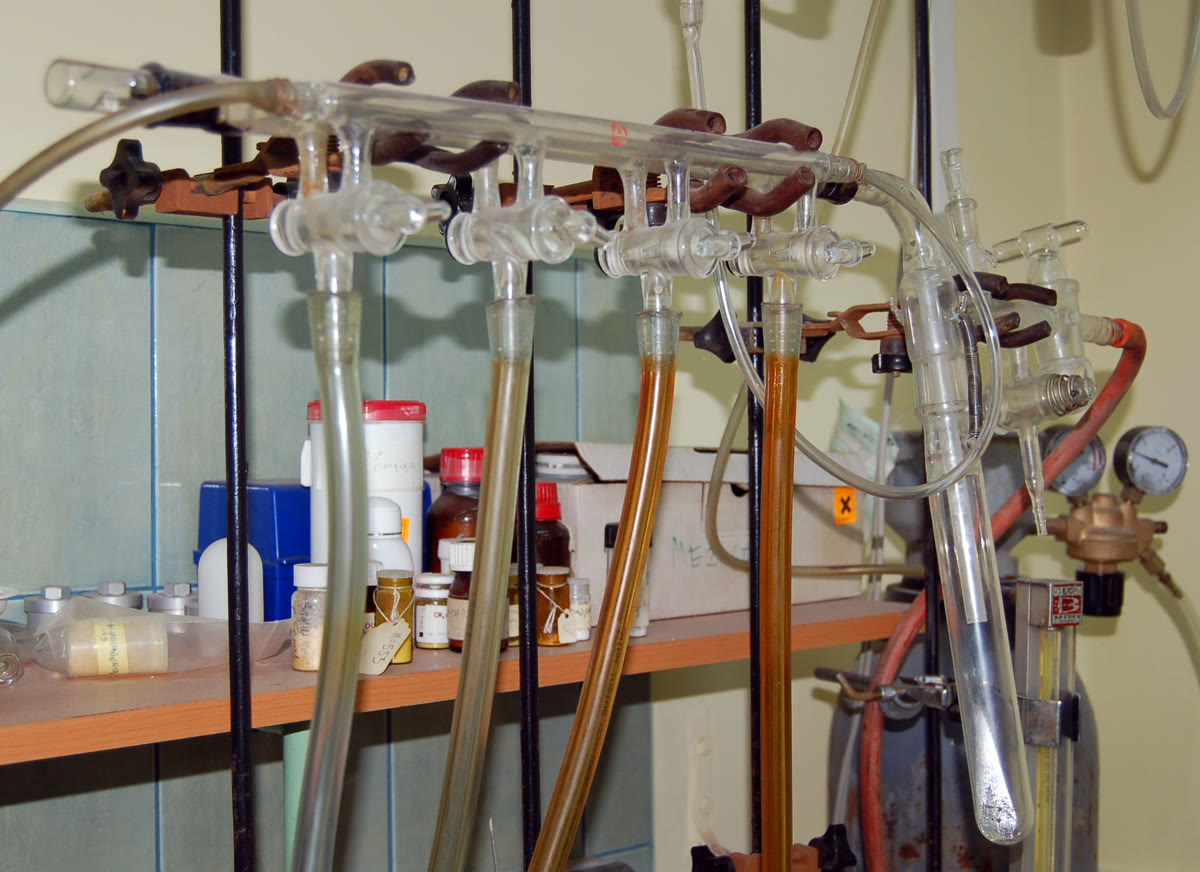
\includegraphics[width=0.46\linewidth]{images/book4/schlenk-line.jpg}

{\small उपयोग में एक \omterm{def:b3:lab-techniques-3:schlenk}{श्लेंक लाइन}: अपनी टोंटियों सहित काँच का नलिका-तंत्र, फ़्लास्कों तक
नलियाँ, और गैस नियामक। छायाचित्र: पोलिमेरेक, CC BY-SA 3.0।}
\end{omfigure}

\section{किसी नए यौगिक का अभिलक्षणन}

\begin{method}[किसी नए यौगिक का अभिलक्षणन]\label{met:b3:lab-techniques-3:characterise}
\begin{enumerate}
  \item शुद्धता: दो निक्षालकों में TLC में एक धब्बा, HPLC या GC में एक शिखर, एक तीक्ष्ण
        गलनांक; यदि द्रव्यमान-शुद्धता आवश्यक हो तो \omterm{def:b3:lab-techniques-3:qnmr}{मात्रात्मक NMR}।
  \item सूत्र: परिकलित द्रव्यमान के कुछ ppm के भीतर HRMS, और समस्थानिक
        प्रतिरूप; या \omterm{def:b3:lab-techniques-3:elemental}{तात्विक विश्लेषण}।
  \item संरचना: संबंधों के लिए 2D प्रयोगों सहित $^1$H और $^{13}$C NMR
        (\cref{ch:b3:advanced-nmr}), क्रियात्मक समूहों के लिए IR; क्रिस्टल उगने पर
        एकल-क्रिस्टल X-किरण संरचना (\cref{ch:b3:x-ray-diffraction})।
  \item त्रिविम रसायन: NOE, युग्मन स्थिरांक, प्रकाशिक घूर्णन, किरैल
        वर्णलेखन द्वारा ee।
  \item प्रत्येक आँकड़े को उसकी परिस्थितियों के साथ, और स्पेक्ट्रमों को \omterm{def:b3:lab-techniques-3:literature}{सहायक
        सूचना} में, प्रस्तुत कीजिए।
\end{enumerate}
\end{method}

\begin{omfigure}
\begin{tikzpicture}[font=\scriptsize, >=Stealth,
  box/.style={draw, rounded corners, align=center, fill=omDef!8, inner sep=3pt, minimum height=8mm}]
  \node[box] (a) at (0,0) {नया यौगिक\\ पृथक};
  \node[box] (b) at (2.85,0) {शुद्ध?\\ TLC, HPLC, गलनांक};
  \node[box] (c) at (5.85,0) {सूत्र\\ HRMS, CHN};
  \node[box] (d) at (8.75,0) {संरचना\\ NMR (1D, 2D), IR};
  \node[box] (e) at (8.75,-1.6) {क्रिस्टल हों तो X-किरण,\\ त्रिविम रसायन};
  \node[box, fill=omMeth!12] (f) at (5.85,-1.6) {संगत?\\ अपरिष्कृत आँकड़ों\\ सहित प्रतिवेदन};
  \node[box, fill=omThm!10] (g) at (2.85,-1.6) {फिर से शोधन\\ (वर्णलेखन,\\ क्रिस्टलन)};
  \draw[->, thick] (a) -- (b); \draw[->, thick] (b) -- node[above, inner sep=1pt] {हाँ} (c);
  \draw[->, thick] (c) -- (d); \draw[->, thick] (d) -- (e); \draw[->, thick] (e) -- (f);
  \draw[->, thick] (b) -- node[left] {नहीं} (g); \draw[->, thick] (g.north west) to[bend left=30] (a.south);
\end{tikzpicture}

{\small किसी नए यौगिक का अभिलक्षणन-कार्यप्रवाह: पहले शुद्धता, फिर
सूत्र, फिर संरचना; प्रत्येक दावा कम से कम दो स्वतंत्र
विधियों पर आधारित होता है, और \omterm{def:b3:lab-techniques-3:notebook}{अपरिष्कृत आँकड़े} प्रतिवेदन के साथ जाते हैं।}
\end{omfigure}

\begin{definition}[तात्विक विश्लेषण]\label{def:b3:lab-techniques-3:elemental}
\emph{तात्विक विश्लेषण}\index{तात्विक विश्लेषण} (दहन विश्लेषण)
किसी नमूने में कार्बन, हाइड्रोजन, नाइट्रोजन और सल्फ़र के द्रव्यमान-प्रतिशत, उसे
ऑक्सीजन में जलाकर और बनने वाली कार्बन डाइऑक्साइड, जल,
डाइनाइट्रोजन और सल्फ़र डाइऑक्साइड को मापकर, निर्धारित करता है।
\end{definition}

\begin{proposition}[सूत्र से द्रव्यमान-प्रतिशत]\label{prop:b3:lab-techniques-3:mass-fractions}
किसी सूत्र $\mathrm{C}_a\mathrm{H}_b\mathrm{N}_c\dots$ के लिए, जिसका मोलर द्रव्यमान $M$ है, कार्बन का द्रव्यमान-प्रतिशत $100\,aA_r(\mathrm C)/M$ है, और इसी प्रकार
अन्य तत्वों के लिए।
\end{proposition}

\begin{proof}
यौगिक के एक मोल में, जिसका द्रव्यमान $M$ है, कार्बन परमाणुओं के $a$ मोल होते हैं, जिनका द्रव्यमान $aA_r(\mathrm C)$ है;
अनुपात, 100 से गुणित, द्रव्यमान-प्रतिशत है।
\end{proof}

% ledger: ea:tolerance, hrms:tolerance
अधिकांश रसायन पत्रिकाएँ संघटन के प्रमाण के रूप में परिकलित मानों के 0.4 प्रतिशत-अंक
के भीतर प्राप्त C, H और N मान, या कुछ ppm (कुछ के लिए 5 ppm) के भीतर
एक HRMS मापन माँगती हैं। एक बड़े अंतरप्रयोगशाला अध्ययन ने पाया कि
शुद्ध नमूने भी आश्चर्यजनक रूप से प्रायः 0.4 मानदंड से चूक जाते हैं, यह स्मरण कराते हुए कि
मानदंड प्रकृति का नियम नहीं है।

\begin{proposition}[HRMS त्रुटि]\label{prop:b3:lab-techniques-3:ppm-error}
किसी मापे गए द्रव्यमान $m_{\text{मापित}}$ की, परिकलित $m_{\text{परिकलित}}$ के विरुद्ध, त्रुटि
$10^6(m_{\text{मापित}} - m_{\text{परिकलित}})/m_{\text{परिकलित}}$ ppm है; किसी आयन के लिए $m_{\text{परिकलित}}$ एकसमस्थानिक द्रव्यमानों से, हटाए गए (या जोड़े गए)
इलेक्ट्रॉनों का द्रव्यमान घटाकर (या जोड़कर), परिकलित किया जाता है।
\end{proposition}

\begin{proof}[परिभाषा से]
ppm त्रुटि प्रति दस लाख भागों में व्यक्त आपेक्षिक अंतर है; आयन का
द्रव्यमान उदासीन सूत्र के द्रव्यमान से इलेक्ट्रॉनों के कारण भिन्न होता है, प्रत्येक \qty{5.486e-4}{u}, जो
कुछ सौ के द्रव्यमानों पर कुछ ppm है।
\end{proof}

\begin{definition}[मात्रात्मक NMR]\label{def:b3:lab-techniques-3:qnmr}
\emph{मात्रात्मक NMR}\index{मात्रात्मक NMR} (qNMR) संकेत-समाकलों से मात्राएँ या
शुद्धताएँ निर्धारित करता है, जो नाभिकों की संख्या के समानुपाती होते हैं
जब स्पेक्ट्रम स्पंदों के बीच पूर्ण विश्रांति के साथ अभिलिखित किया जाए, नमूने के साथ
तौले गए ज्ञात शुद्धता के एक आंतरिक मानक के विरुद्ध।
\end{definition}

\begin{proposition}[qNMR शुद्धता]\label{prop:b3:lab-techniques-3:qnmr}
द्रव्यमान $m_x$ के एक नमूने के लिए, जिसे द्रव्यमान $m_s$ और शुद्धता $P_s$ वाले मानक के साथ तौला गया हो, और जिसके संकेतों
के समाकल $I_x$ और $I_s$ हों, जो $N_x$ और $N_s$ प्रोटॉनों से आते हैं,
\[
  P_x = \frac{I_x}{I_s}\,\frac{N_s}{N_x}\,\frac{M_x}{M_s}\,\frac{m_s}{m_x}\,P_s.
\]
\end{proposition}

\begin{proof}
समाकल प्रोटॉनों की संख्याओं के समानुपाती हैं: $I_x/I_s = (N_xn_x)/(N_sn_s)$।
$n_x = P_xm_x/M_x$ और $n_s = P_sm_s/M_s$ के साथ, $P_x$ के लिए हल करने पर सूत्र मिलता है।
\end{proof}

\begin{omfigure}
\begin{tikzpicture}
\begin{axis}[width=0.8\linewidth, height=5.0cm, x dir=reverse, xmin=3.0, xmax=7.0, ymin=-0.05, ymax=1.15, clip=false,
  axis x line=bottom, axis y line=none, xlabel={$\delta$ / ppm}, tick label style={font=\scriptsize}, label style={font=\small}]
\addplot[color=omDef, thick] table[x=ppm, y=y] {figdata/out/bachelor-3-qnmr.dat};
\node[font=\scriptsize, anchor=south] at (axis cs:6.09,0.33) {मानक, ArH (3 H)};
\node[font=\scriptsize, anchor=east] at (axis cs:4.20,0.98) {फ़ेरोसीन (10 H)};
\node[font=\scriptsize, anchor=west, align=left] at (axis cs:3.72,0.70) {मानक,\\ $\ce{OCH3}$ (9 H)};
\end{axis}
\end{tikzpicture}

{\small आंतरिक मानक के रूप में 1,3,5-ट्राइमेथॉक्सीबेंज़ीन के साथ तौले गए फ़ेरोसीन नमूने का
संश्लिष्ट प्रोटॉन स्पेक्ट्रम (मॉडल: 98.0\,\% शुद्धता वाले नमूने का 20.0 mg,
मानक का 15.0 mg)। समाकल प्रोटॉनों की संख्या और प्रत्येक यौगिक की
मात्रा के गुणनफल के समानुपाती हैं; फ़ेरोसीन एकक का
मानक के ऐरोमैटिक एकक से अनुपात शुद्धता देता है।}
\end{omfigure}

\section{किसी शोध-परिणाम की सांख्यिकी}

\begin{definition}[सार्थकता परीक्षण]\label{def:b3:lab-techniques-3:tests}
\emph{सार्थकता परीक्षण}\index{सार्थकता परीक्षण} यह तय करता है कि आँकड़े किसी
\emph{शून्य परिकल्पना}\index{शून्य परिकल्पना} के, जो सामान्यतः यह होती है कि
कोई अंतर या कोई प्रभाव नहीं है, संगत हैं या नहीं, उसे ग़लती से अस्वीकार करने के जोखिम के
एक चुने हुए स्तर पर (प्रायः 5\,\%)।
\end{definition}

\begin{theorem}[दो-प्रतिदर्श $t$ परीक्षण]\label{thm:b3:lab-techniques-3:t-test}
समान मानक विचलन वाले सामान्य बंटनों से लिए गए $n_1$ और $n_2$ स्वतंत्र मापनों के
दो समुच्चयों के लिए, जिनके माध्य $\bar x_1$, $\bar x_2$ और संयुक्त
मानक विचलन $s_p$ हों, सांख्यिकी $t = (\bar x_1 - \bar x_2)/(s_p\sqrt{1/n_1 + 1/n_2})$ स्टूडेंट नियम का पालन करती है,
$n_1 + n_2 - 2$ स्वातंत्र्य कोटियों के साथ, जब दोनों वास्तविक माध्य बराबर हों। \admitted
\end{theorem}

\begin{proposition}[$F$ परीक्षण]\label{prop:b3:lab-techniques-3:f-test}
उन्हीं मान्यताओं के अंतर्गत, दो प्रतिदर्श प्रसरणों का अनुपात $F = s_1^2/s_2^2$
फ़िशर नियम का पालन करता है, $(n_1 - 1, n_2 - 1)$ स्वातंत्र्य कोटियों के साथ, जब वास्तविक प्रसरण बराबर हों।
\admitted
\end{proposition}

\begin{method}[क्या नई लब्धि बेहतर है?]\label{met:b3:lab-techniques-3:compare-means}
\begin{enumerate}
  \item दोनों प्रक्रियाओं को समान परिस्थितियों में कई बार दोहराइए; प्रत्येक
        परिणाम अभिलिखित कीजिए।
  \item पहले प्रसारों की तुलना कीजिए ($F$ परीक्षण); यदि वे समान हों, तो उन्हें संयुक्त कीजिए:
        $s_p^2 = [(n_1 - 1)s_1^2 + (n_2 - 1)s_2^2]/(n_1 + n_2 - 2)$।
  \item $t$ परिकलित कीजिए और $|t|$ की तुलना, चुने हुए स्तर पर, $n_1 + n_2 - 2$ स्वातंत्र्य
        कोटियों के स्टूडेंट गुणांक से कीजिए।
  \item अधिक: अंतर सार्थक है। कम: आँकड़े कोई अंतर नहीं दर्शाते,
        जो यह सिद्ध नहीं करता कि कोई अंतर नहीं है।
\end{enumerate}
\end{method}

किसी संदिग्ध मान को कभी इसलिए नहीं हटाया जाता कि वह असुविधाजनक है। बहिर्वर्ती परीक्षण
उसे चिह्नित करते हैं, पर निर्णय नोटबुक पर टिका होता है: कोई अभिलिखित कारण (तौल की
त्रुटि, संदूषित फ़्लास्क) उसे अस्वीकार करना उचित ठहराता है; उसके बिना, मान रखा जाता है,
या प्रयोग दोहराया जाता है।

\section{नोटबुक, शोध आँकड़े और साहित्य}

\begin{definition}[नोटबुक और अपरिष्कृत आँकड़े]\label{def:b3:lab-techniques-3:notebook}
\emph{प्रयोगशाला नोटबुक}\index{प्रयोगशाला नोटबुक} किए गए प्रयोगों का, जैसे वे
किए गए वैसे ही, दिनांकित, सतत, अपरिवर्तित अभिलेख है। \emph{अपरिष्कृत
आँकड़े}\index{अपरिष्कृत आँकड़े} किसी भी प्रसंस्करण से पहले मापनों के मूल अभिलेख (उपकरण-फ़ाइलें,
तौल-पर्चियाँ, स्पेक्ट्रम) हैं।
\end{definition}

\begin{method}[नोटबुक प्रविष्टि लिखना]\label{met:b3:lab-techniques-3:notebook}
\begin{enumerate}
  \item दिनांक, शीर्षक, उद्देश्य, और पिछले संबंधित प्रयोग का संदर्भ।
  \item मात्राओं (द्रव्यमान, आयतन, मोल, तुल्यांक), अभिकर्मकों के स्रोतों
        और बैचों, और \omterm{def:b3:lab-techniques-3:assessment}{जोखिम मूल्यांकन} सहित अभिक्रिया-योजना।
  \item जो किया गया और देखा गया, क्रम से और उसी समय, जिसमें वह भी शामिल हो जो
        ग़लत हुआ; कभी मिटाइए नहीं, ऐसे काटिए कि मूल पढ़ा जा सके।
  \item परिणाम: लब्धियाँ, अपरिष्कृत आँकड़ा-फ़ाइलों के नाम, और एक निष्कर्ष; हस्ताक्षर कीजिए।
\end{enumerate}
\end{method}

\begin{definition}[FAIR आँकड़े]\label{def:b3:lab-techniques-3:fair}
% ledger: fair:year
\emph{FAIR आँकड़े}\index{FAIR आँकड़े} वे शोध आँकड़े हैं जो खोजने योग्य,
सुलभ, अंतर्प्रचालनीय और पुनःप्रयोज्य हों (अंग्रेज़ी आद्याक्षरों से FAIR): समृद्ध मेटाडेटा और एक
स्थायी पहचानकर्ता के साथ वर्णित, मानक प्रोटोकॉल से पुनःप्राप्य, खुले प्रारूपों में,
स्पष्ट लाइसेंस और उद्गम के साथ।
\end{definition}

\begin{definition}[शोध सत्यनिष्ठा]\label{def:b3:lab-techniques-3:integrity}
\emph{शोध सत्यनिष्ठा}\index{शोध सत्यनिष्ठा} शोध का ईमानदार और
पारदर्शी संचालन और प्रतिवेदन है। इसके सबसे गंभीर उल्लंघन
\emph{मनगढ़ंत रचना}\index{मनगढ़ंत रचना} (आँकड़ों का आविष्कार), \emph{मिथ्याकरण}\index{मिथ्याकरण}
(आँकड़ों, चित्रों या प्रक्रियाओं को बदलना) और \emph{साहित्यिक चोरी}\index{साहित्यिक चोरी}
(दूसरों के कार्य को अपना बताना) हैं।
\end{definition}

\begin{definition}[साहित्य]\label{def:b3:lab-techniques-3:literature}
\emph{प्राथमिक साहित्य}\index{प्राथमिक साहित्य} मौलिक
शोध का प्रतिवेदन करता है (लेख, पेटेंट, शोध-प्रबंध); \emph{द्वितीयक
साहित्य}\index{द्वितीयक साहित्य} उसकी समीक्षा और व्यवस्था करता है (समीक्षाएँ,
पुस्तिकाएँ, आँकड़ा-संचय), और पाठ्यपुस्तकें एक तृतीयक स्तर बनाती हैं। \emph{सहकर्मी
समीक्षा}\index{सहकर्मी समीक्षा} प्रकाशन से पहले स्वतंत्र विशेषज्ञों द्वारा किसी पांडुलिपि का
मूल्यांकन है। किसी लेख की \emph{सहायक सूचना}\index{सहायक सूचना}
में कार्य को दोहराने और जाँचने के लिए आवश्यक प्रायोगिक विवरण और आँकड़े
होते हैं।
\end{definition}

\begin{method}[किसी प्रकाशित प्रक्रिया को पढ़ना]\label{met:b3:lab-techniques-3:read-paper}
\begin{enumerate}
  \item केवल सार और योजना ही नहीं, प्रायोगिक खंड और \omterm{def:b3:lab-techniques-3:literature}{सहायक सूचना}
        पढ़िए।
  \item पैमाना, सांद्रताएँ, ताप, समय और उपचार-पश्चात् प्रक्रिया जाँचिए; जो
        छूटा है उसे नोट कीजिए।
  \item उत्पादों के अभिलक्षणन को ऊपर की विधि के विरुद्ध जाँचिए।
  \item ऐसे बाद के शोधपत्र खोजिए जिन्होंने प्रक्रिया का उपयोग किया या उसे सुधारा; पहले इसे
        छोटे पैमाने पर चलाइए।
\end{enumerate}
\end{method}

संरचना और अभिक्रिया आँकड़ा-संचय \omterm{def:b3:lab-techniques-3:literature}{प्राथमिक साहित्य} को यौगिक और
रूपांतरण के अनुसार अनुक्रमित करते हैं, और उनमें शब्दों के बजाय कोई संरचना या अभिक्रिया
बनाकर खोज की जाती है।

\section{किसी नई प्रक्रिया का जोखिम मूल्यांकन}

\begin{definition}[जोखिम मूल्यांकन]\label{def:b3:lab-techniques-3:assessment}
किसी प्रक्रिया का \emph{जोखिम मूल्यांकन}\index{जोखिम मूल्यांकन} उसके
संकटों की पहचान करता है, नियोजित परिस्थितियों में हानि की संभावना और गंभीरता का अनुमान लगाता है,
और ऐसे नियंत्रण तय करता है जो जोखिम को स्वीकार्य स्तर तक घटाएँ।
\emph{नियंत्रणों का पदानुक्रम}\index{नियंत्रणों का पदानुक्रम} उन्हें सबसे अधिक से
सबसे कम प्रभावी तक श्रेणीबद्ध करता है: उन्मूलन, प्रतिस्थापन, अभियांत्रिक नियंत्रण,
प्रशासनिक नियंत्रण, व्यक्तिगत सुरक्षा उपकरण।
\end{definition}

\begin{omfigure}
\begin{tikzpicture}[font=\scriptsize]
  \foreach \i/\lab/\col in {0/उन्मूलन: संकट को हटाइए/omMeth!40, 1/प्रतिस्थापन: कम ख़तरनाक अभिकर्मक/omMeth!28, 2/अभियांत्रिक: धूम-हुड{,} ग्लवबॉक्स{,} कवच/omDef!22, 3/प्रशासनिक: प्रक्रियाएँ{,} प्रशिक्षण/omProp!22, 4/व्यक्तिगत सुरक्षा उपकरण/omThm!22} {
    \pgfmathsetmacro\w{5.4-0.95*\i}
    \fill[\col] ({-\w/2},{-0.75*\i}) -- ({\w/2},{-0.75*\i}) -- ({\w/2-0.475},{-0.75*\i-0.7}) -- ({-\w/2+0.475},{-0.75*\i-0.7}) -- cycle;
    \node[anchor=west] at (3.0,{-0.75*\i-0.35}) {\lab};
    \draw[black!30] ({\w/2-0.2},{-0.75*\i-0.35}) -- (2.95,{-0.75*\i-0.35});
  }
  \node[anchor=east, align=right] at (-2.9,-0.35) {सबसे अधिक\\ प्रभावी};
  \node[anchor=east, align=right] at (-2.9,-3.35) {सबसे कम\\ प्रभावी};
  \draw[->, black!50] (-3.3,-0.85) -- (-3.3,-2.85);
\end{tikzpicture}

{\small \omterm{def:b3:lab-techniques-3:assessment}{नियंत्रणों का पदानुक्रम}, एक उलटे पिरामिड के रूप में: संकट को हटाना या बदलना
सबकी, सदैव, रक्षा करता है; सुरक्षा उपकरण केवल उसे पहनने वाले की रक्षा करता है,
और केवल तभी जब वह पहना हुआ और अक्षत हो।}
\end{omfigure}

\begin{definition}[पेरॉक्साइड-निर्माता]\label{def:b3:lab-techniques-3:peroxide}
\emph{पेरॉक्साइड-निर्माता}\index{पेरॉक्साइड-निर्माता} ऐसा यौगिक है, जैसे डाइएथिल
ईथर, टेट्राहाइड्रोफ़्यूरान या 1,4-डाइऑक्सेन, जो भंडारण में, विशेषकर खोलने के बाद और प्रकाश में,
वायु के साथ धीरे-धीरे विस्फोटक पेरॉक्साइड बनाता है।
\end{definition}

\begin{method}[किसी नई प्रक्रिया के जोखिमों का मूल्यांकन]\label{met:b3:lab-techniques-3:risk-assessment}
\begin{enumerate}
  \item प्रत्येक पदार्थ (अभिकर्मक, विलायक, उत्पाद, उप-उत्पाद, मुक्त
        गैसें) को सुरक्षा आँकड़ा पत्रक से उसके संकटों के साथ सूचीबद्ध कीजिए।
  \item संक्रियाओं और उनकी परिस्थितियों (तापन, दाब, पैमाना,
        शमन, अपशिष्ट) को सूचीबद्ध कीजिए; पैमाना बढ़ाने से पहले मुक्त ऊष्मा और रुद्धोष्म ताप-वृद्धि
        का अनुमान लगाइए।
  \item प्रत्येक संकट के लिए पदानुक्रम में नीचे की ओर नियंत्रण चुनिए; आपातकालीन
        प्रतिक्रिया (छलकाव, आग, अनावरण) और अपशिष्ट-मार्ग की योजना बनाइए।
  \item इसे लिखिए, इसकी जाँच करवाइए, और पहली बार चलाने के बाद इसकी समीक्षा कीजिए।
\end{enumerate}
\end{method}

\begin{safety}{\ghs[0.62cm]{GHS02}\ghs[0.62cm]{GHS05}\ghs[0.62cm]{GHS07}\ghs[0.62cm]{GHS08}}
% ledger: ghs4:BuLi, ghs4:Et2O, ghs4:THF
ब्यूटिललिथियम विलयन: स्वतःज्वलनशील, जल के साथ ज्वलनशील गैस मुक्त करते हुए तीव्र अभिक्रिया करते हैं,
गंभीर दाह उत्पन्न करते हैं; केवल अक्रिय गैस के अधीन, पास में शुष्क
रेत की बाल्टी रखकर और निकट कोई जल न होने पर, सँभाले जाते हैं। सोडियम हाइड्राइड भी जल और नमी के साथ
हाइड्रोजन मुक्त करता है, और तेल में परिक्षेपण के रूप में प्रयुक्त होता है। डाइएथिल
ईथर और THF अत्यधिक ज्वलनशील \omterm{def:b3:lab-techniques-3:peroxide}{पेरॉक्साइड-निर्माता} हैं: खोलने पर दिनांकित, आसवन या वाष्पन से पहले
पेरॉक्साइडों के लिए परीक्षित, और निर्धारित समय पर त्याग दिए जाते हैं।
\end{safety}

\begin{history}[श्लेंक के काँच के उपकरण]
1910 के दशक में कार्ब-क्षारधातु यौगिकों और मूलकों का अध्ययन करते हुए विल्हेम श्लेंक ने
ऐसे फ़्लास्क और तकनीकें अभिकल्पित कीं जिनसे वे उन्हें बिना वायु के सँभाल सके; लाइन और
फ़्लास्क आज भी उनका नाम धारण करते हैं। पहले \omterm{def:b3:lab-techniques-3:schlenk}{ग्लवबॉक्स}
1940 के दशक में रेडियोधर्मी पदार्थों के लिए बनाए गए और शीघ्र ही \omterm{def:b3:lab-techniques-3:air-sensitive}{वायु-संवेदी यौगिकों} के साथ कार्य करने वाले
रसायनज्ञों ने उन्हें अपना लिया।
\end{history}

\section{अभ्यास}

\begin{exercise}[$\star$]\label{exo:b3:lab-techniques-3:1}
एक फ़्लास्क को \qty{0.50}{mbar} तक निर्वातित करके आर्गन से \qty{1013}{mbar} तक तीन बार पुनः भरा जाता है। सिद्धांततः
मूल वायु का कितना अंश शेष रहता है? वास्तव में परिणाम को क्या सीमित करता है?
\end{exercise}

\begin{exercise}[$\star$]\label{exo:b3:lab-techniques-3:2}
एक ब्यूटिललिथियम विलयन का अनुमापांक \qty{1.48}{mol/L} है। \qty{20.0}{mmol} देने के लिए कितना आयतन
स्थानांतरित करना होगा?
\end{exercise}

\begin{exercise}[$\star$]\label{exo:b3:lab-techniques-3:3}
% ledger: mass:C12, mass:H1, mass:Fe56, const4:me.u, hrms:tolerance
फ़ेरोसीन मूलक धनायन $\ce{C10H10Fe+}$ का यथातथ द्रव्यमान एकसमस्थानिक द्रव्यमानों
($^{12}$C ठीक 12, $^1$H 1.00782503, $^{56}$Fe 55.93493633, इलेक्ट्रॉन \qty{5.486e-4}{u}) से परिकलित कीजिए, और
186.0129 के मापे गए मान की ppm में त्रुटि।
\end{exercise}

\begin{exercise}[$\star$]\label{exo:b3:lab-techniques-3:4}
प्राथमिक, द्वितीयक या तृतीयक साहित्य के रूप में वर्गीकृत कीजिए: एक समीक्षा लेख, एक
नए संश्लेषण का प्रतिवेदन देने वाला शोध-पत्रिका लेख, एक पेटेंट, भौतिक
स्थिरांकों की एक पुस्तिका, एक शोध-प्रबंध, एक पाठ्यपुस्तक।
\end{exercise}

\begin{exercise}[$\star\star$]\label{exo:b3:lab-techniques-3:5}
% ledger: ea:tolerance
कैफ़ीन, $\ce{C8H10N4O2}$, के C, H और N द्रव्यमान-प्रतिशत परिकलित कीजिए, और तय कीजिए कि प्राप्त
मान C 49.31, H 5.22, N 28.71\,\% सामान्य 0.4-अंक मानदंड को पूरा करते हैं या नहीं।
\end{exercise}

\begin{exercise}[$\star\star$]\label{exo:b3:lab-techniques-3:6}
\qty{170.0}{mg} डाइफ़ेनिलऐसीटिक अम्ल ($\ce{C14H12O2}$) के एक नमूने को पीले अंत्य बिंदु तक पहुँचने के लिए \qty{0.54}{mL} ब्यूटिललिथियम विलयन
चाहिए। अनुमापांक परिकलित कीजिए।
\end{exercise}

\begin{exercise}[$\star\star$]\label{exo:b3:lab-techniques-3:7}
एक पुरानी प्रक्रिया ने 72, 75, 71, 74 और 73\,\% लब्धियाँ दीं; एक संशोधित प्रक्रिया ने 76, 78, 75, 77 और
79\,\%। 95\,\% पर 8 स्वातंत्र्य कोटियों के लिए स्टूडेंट गुणांक 2.31 के साथ (अभ्यास के आँकड़े),
क्या सुधार सार्थक है?
\end{exercise}

\begin{exercise}[$\star\star$]\label{exo:b3:lab-techniques-3:8}
दो विधियाँ छह-छह परिणाम देती हैं, जिनके मानक विचलन 0.80 और 0.30 हैं (समान
इकाइयाँ)। 95\,\% पर (5, 5) स्वातंत्र्य कोटियों के लिए 5.05 के क्रांतिक $F$ के साथ (अभ्यास के
आँकड़े), क्या उनकी परिशुद्धताएँ भिन्न हैं?
\end{exercise}

\begin{exercise}[$\star\star$]\label{exo:b3:lab-techniques-3:9}
किसी प्रयोगशाला की THF और डाइएथिल ईथर की बोतलों के लिए भंडारण और परीक्षण की एक योजना
प्रस्तावित कीजिए।
\end{exercise}

\begin{exercise}[$\star\star\star$]\label{exo:b3:lab-techniques-3:10}
एक विद्यार्थी 50 g पैमाने पर DMF में 60 °C पर सोडियम हाइड्राइड से किसी ऐल्कोहॉल को
विप्रोटॉनित करने की योजना बनाता है। संकटों की पहचान कीजिए (इस विलायक के
क्षारक के साथ तापीय संकटों सहित) और पदानुक्रम में नीचे की ओर नियंत्रण चुनिए।
\end{exercise}

\begin{exercise}[$\star\star\star$]\label{exo:b3:lab-techniques-3:11}
$I_x$, $I_s$ (प्रत्येक 0.50\,\%), $m_x$ और $m_s$ (\qty{0.010}{mg}, 20.0
और 15.0 mg पर) और $P_s$ (0.10\,\%) की आपेक्षिक मानक अनिश्चितताओं को qNMR सूत्र से होकर संचरित कीजिए, और $P_x$ की आपेक्षिक अनिश्चितता बताइए।
कौन-सा पद प्रभावी है?
\end{exercise}

\begin{exercise}[$\star\star\star$]\label{exo:b3:lab-techniques-3:12}
पाँच अनुमापन 81.2, 82.0, 80.6, 81.5 और 89.0 (mL में) देते हैं। एक डिक्सन परीक्षण
0.71 के क्रांतिक मान के विरुद्ध $Q = 0.83$ देता है (अभ्यास के आँकड़े)। क्या अंतिम मान
अस्वीकार किया जाना चाहिए? समझाइए कि आप पहले क्या जाँचेंगे।
\end{exercise}

\section{समस्या: फ़्लास्क से शोधपत्र तक}

\begin{problem}[{सप्ताहांत समस्या --- फ़्लास्क से शोधपत्र तक, एक नया वायु-संवेदी
यौगिक: नाइट्रोजन के अधीन फ़ेरोसीन का संश्लेषण, उसका अभिलक्षणन, मात्रात्मक NMR द्वारा उसकी
शुद्धता, और प्रक्रिया का जोखिम मूल्यांकन}]
\label{pb:b3:lab-techniques-3:1}
% ledger: aw:C, aw:H, aw:Fe, aw:Cl, aw:O, mass:C12, mass:H1, mass:Fe56, const4:me.u, ghs4:ferrocene
समस्या के आँकड़े। निर्जल आयरन(II) क्लोराइड (5.00 g) नाइट्रोजन के अधीन सोडियम
साइक्लोपेन्टाडाइएनाइड (दो तुल्यांक, THF में साइक्लोपेन्टाडाईन और सोडियम हाइड्राइड से)
से अभिक्रिया करता है; 5.86 g नारंगी फ़ेरोसीन, $\ce{Fe(C5H5)2}$, पृथक किया जाता है। फ़्लास्कों को
\qty{0.10}{mbar} तक तीन चक्रों द्वारा, \qty{1000}{mbar} से आरंभ करके, शोधित किया जाता है। HRMS $m/z$ 186.0129 देता है, $\ce{M+}$ के लिए; \omterm{def:b3:lab-techniques-3:elemental}{तात्विक
विश्लेषण} C 64.41, H 5.47\,\%। $\ce{CDCl3}$ में फ़ेरोसीन 4.16 ppm पर एक एकक देता है (10 H)। qNMR के लिए,
नमूने के 20.0 mg और 1,3,5-ट्राइमेथॉक्सीबेंज़ीन के 15.0 mg (शुद्धता 99.9\,\%, 6.09 ppm पर ऐरोमैटिक
एकक, 3 H) $I_x/I_s = 3.942$ देते हैं, प्रत्येक समाकल के लिए 0.50\,\%,
प्रत्येक द्रव्यमान के लिए \qty{0.010}{mg} और $P_s$ के लिए 0.10\,\% की आपेक्षिक मानक अनिश्चितताओं के साथ।

\medskip\noindent\textbf{भाग I --- नाइट्रोजन के अधीन संश्लेषण।}
\begin{enumerate}
  \item संश्लेषण का समीकरण लिखिए।
  \item अभिक्रिया को बिना वायु के क्यों चलाना चाहिए?
  \item फ़ेरोसीन का सैद्धांतिक द्रव्यमान और लब्धि परिकलित कीजिए।
  \item तीन शोधन-चक्रों के बाद शेष वायु का अंश परिकलित कीजिए।
  \item साइक्लोपेन्टाडाईन उसके द्वितय से कैसे प्राप्त किया जाता है, और उसे तुरंत क्यों प्रयुक्त करना चाहिए?
  \item सोडियम हाइड्राइड अंशों में क्यों मिलाया जाता है?
\end{enumerate}

\medskip\noindent\textbf{भाग II --- अभिलक्षणन।}
\begin{enumerate}[resume]
  \item $\ce{M+}$ का यथातथ द्रव्यमान और मापन की ppm में त्रुटि परिकलित कीजिए।
  \item C और H द्रव्यमान-प्रतिशत परिकलित कीजिए और विश्लेषण से तुलना कीजिए।
  \item फ़ेरोसीन एक ही $^1$H संकेत क्यों दर्शाता है?
  \item $^{13}$C NMR क्या दर्शाएगा?
  \item कौन-सी अतिरिक्त विधि सैंडविच संरचना को सिद्ध करेगी?
  \item क्या बनने के बाद फ़ेरोसीन स्वयं वायु-संवेदी है? इसकी तुलना इसके पूर्वगामियों से कीजिए।
\end{enumerate}

\medskip\noindent\textbf{भाग III --- qNMR द्वारा शुद्धता।}
\begin{enumerate}[resume]
  \item यहाँ मानक के रूप में 1,3,5-ट्राइमेथॉक्सीबेंज़ीन क्यों चुना जाए?
  \item समाकलों के मात्रात्मक होने के लिए NMR अभिग्रहण को किस बात की गारंटी देनी चाहिए?
  \item फ़ेरोसीन और मानक के मोलर द्रव्यमान परिकलित कीजिए।
  \item नमूने की शुद्धता परिकलित कीजिए।
  \item उसकी आपेक्षिक और निरपेक्ष मानक अनिश्चितता परिकलित कीजिए।
  \item क्या \omterm{def:b3:lab-techniques-3:elemental}{तात्विक विश्लेषण} इस शुद्धता से संगत है?
\end{enumerate}

\medskip\noindent\textbf{भाग IV --- जोखिम और एक अंतिम मापन।}
\begin{enumerate}[resume]
  \item प्रक्रिया के संकटों की सूची बनाइए।
  \item सोडियम हाइड्राइड और THF के लिए नियंत्रण चुनिए।
  \item अंत में अधिक सोडियम हाइड्राइड को कैसे नष्ट किया जाना चाहिए?
  \item फ़ेरोसीन का चक्रीय \omterm{def:b3:electrode-kinetics:cv}{वोल्टामोग्राम} क्या दर्शाता है, और विद्युतरसायन में फ़ेरोसीन
        संदर्भ के रूप में क्यों प्रयुक्त होता है?
  \item नोटबुक प्रविष्टि और \omterm{def:b3:lab-techniques-3:literature}{सहायक सूचना} में क्या होना चाहिए?
  \item अपरिष्कृत स्पेक्ट्रमों को खुले प्रारूप में संग्रहित क्यों किया जाना चाहिए?
  \item परिणाम बताइए: फ़ेरोसीन नमूने की qNMR शुद्धता, उसकी मानक
        अनिश्चितता सहित।
\end{enumerate}
\end{problem}
